%MIT OpenCourseWare: https://ocw.mit.edu
%RES.18-011 Algebra I Student Notes, Fall 2021
%License: Creative Commons BY-NC-SA 
%For information about citing these materials or our Terms of Use, visit: https://ocw.mit.edu/terms.

\section{Group Actions}

Today, we will discuss group operations or actions\footnote{They are different terms for the same idea. Artin uses group operations, while Professor Maulik prefers to call them group actions.} on a set.
\begin{qq}
How can a group be seen as a group of transformations?%\footnote{Like matrices, our motivating example all the way back from the first lecture!}
\end{qq}

\subsection{Review}
Last time, we finished talking about (discrete) subgroups of isometries of the plane. Finite subgroups of $M_2$ are isomorphic to $C_n$ or $D_n,$ and there are only finitely many isomorphism classes of infinite discrete subgroups of $M_2$.\footnote{In fact, with \emph{any} metric space, which is a set with some distance on it (as discussed in 18.100, for example), it's possible to consider isometries, distance-preserving transformations, in the same way as we considered the plane $\RR^2.$ Depending on the metric space, the groups can look very different! One example of this is the hyperbolic plane, which is the upper half-plane of $\RR^2$ with a non-Euclidean metric, or distance, on it, and the discrete subgroups of isometries on it. There are infinitely many discrete subgroups of isometries on it, even though it is 2-dimensional, just like $\RR^2.$ The question of why it is so different from the $\RR^2$ case is really a geometry question, rather than an algebra question.} 

It is also possible to go up a dimension and classify discrete subgroups of isometries of $\RR^3$, although it is more complicated; there are 200 or so. 



\subsection{Motivating Examples}
The idea of a group action will generalize and make more abstract an idea that has been present throughout the class so far. Let's start with the following motivating example. 
\begin{example}[$GL_n$]
Given $g \in GL_n(\RR)$ and a column vector $v \in \RR^n,$ the matrix $g$ can be seen as a transformation on $\RR^n,$ taking $v \mapsto g(v) \in \RR^n.$ 

The data of $GL_n(\RR)$ acting on $\RR^n$ can be packaged together by a map 
\begin{align*}
    GL_n(\RR) \by \RR^n &\rto \RR^n \\
    (g, \vvv) &\mto g(\vvv).
\end{align*}
\end{example}

The same principle applies to $S_n,$ the group of permutations on $\{1, \cdots, n\}$.
\begin{example}[$S_n$]
The symmetric group $S_n$ can also be viewed as acting on a set. More or less by definition, given a number between 1 and n, and a permutation, it's possible to spit out the result of permutation acting on that number. So $S_n$ permutes the set $[n] = \{1, \cdots, n\}.$
This gives us another mapping encoding this information:
\begin{align*}
    S_n \by \{1, \cdots, n\} &\rto \{1, \cdots, n\} \\
    (\sigma, i) &\mto \sigma(i).
\end{align*} 
\end{example}

Our last example is one we have been considering for the past few lectures.
\begin{example}
The set $M_2$, isometries of 2-space, acts on $\RR^2:$ given some vector in the plane and some isometry, the isometry will return some other vector in the plane. This information is again encoded by a mapping
\begin{align*}
    M_2(\RR) \by \RR^2 &\rto \RR^2 \\
    (f, \vec{x}) &\mto f(\vec{x}). 
\end{align*}
\end{example}

\subsection{What is a group action?}
These are all examples of group operations on a set, and they motivate the following definition of a group operation in general.
\begin{definition}
Given a group $G$ and a set $S,$ a \textbf{group action}\footnote{or group operation} on a set $S$ is a mapping 
\begin{align*}
    G \by S &\rto S \\
    (g, s) &\mto gs.
\end{align*}
It must satisfy the following axioms:
\begin{itemize}
    \item The identity maps every element of the set back to itself: $es = s$ for all $s \in S.$\footnote{This corresponds to the identity multiplication rule.}
    \item The mapping must respect the group multiplication: $(gh)s = g(hs)$ for $s \in S$ and $g, h \in G.$\footnote{This corresponds to the associativity rule.}
\end{itemize}
\end{definition}

Essentially, given an element $g \in G$ and $s \in S,$ the mapping returns another element of $S$ depending on $g,$ and the mapping must respect the group structure on $G.$ All of the groups that we have seen so far show up as symmetries of some set, maybe preserving some extra structure, so all the groups that we usually think about already come with an action on some set $S.$ Furthermore, a group $G$ can act on many different sets at the same time in different ways, which gives insight into the group itself.

Let's look at a couple of examples.
\begin{example}[$S_4$]
The symmetric group $S_4,$ permutations on 4 elements, acts on $S = \{1, 2, 3, 4\}$. It can \emph{also} act on a different set, $T = \{\text{unordered pairs in } S \} = \{(12),(13), (14), (23), (24), (34)\}.$ The set $T$ has 6 elements, and $S_4$ acts on $T$ as well as acting on $S.$ Given a permutation $\sigma \in S_4,$ and an unordered pair $\{i, j\},$ it acts by taking
\[
\sigma(\{i, j\}) = \{\sigma(i), \sigma(j)\}
\]
for a permutation $\sigma \in S_4.$ 
\end{example}

So the group action on $S$ leads to a different group action on a different set, $T.$ The existence of a group action on a given set actually yields a lot of information about the group $G,$ as will be explored in the next few lectures. Let's see a different example.

\begin{example}[$D_2$]\label{grp action d2}
Let $G = D_2,$ which contains rotation by $\pi$ as well as reflection across the $x$-axis (and then reflection across the $y$-axis.) As a subgroup of $O_2,$\footnote{$2 \by 2$ orthogonal matrices}, $D_2$ will act on all of $\RR^2.$ It also acts on the set $S$ consisting of the vertices of a square and a diamond, as well as the center. 

\begin{center}
    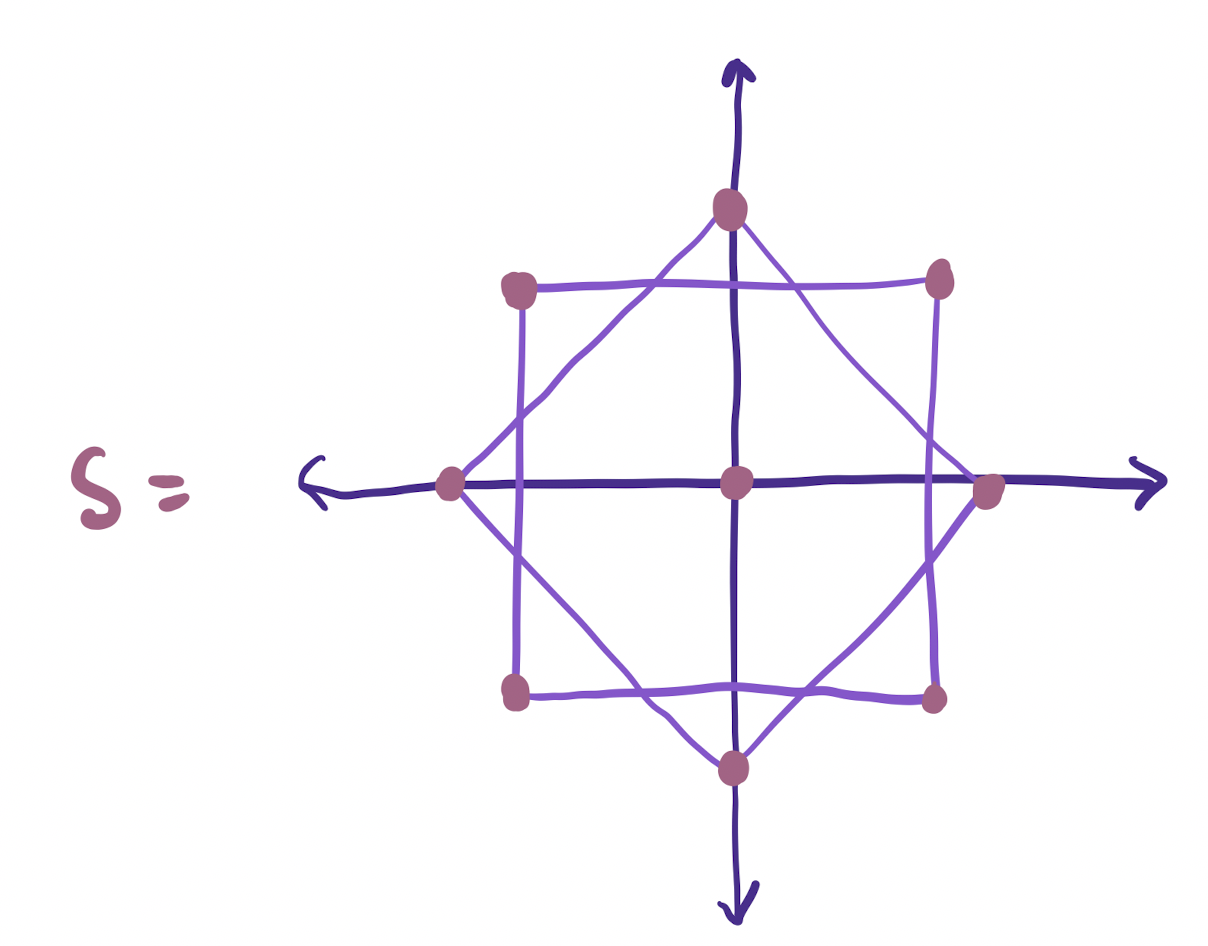
\includegraphics[width=5cm]{Lecture Files and Images/lec17-S.png}
\end{center}
\end{example}

A group $G$ can also act on itself viewed as a set.
\begin{example}
Given a group $G,$ there is a mapping
\begin{align*}
    G \by G &\rto G \\
    (g, g') &\mto gg',
\end{align*}
and this is a valid group action. 
\end{example}

When $G$ acts on itself, the first $G$ in $G \by G$ is seen as a group, while the second $G$ is seen as a set, since the axioms of a group action don't care about the group operation on the second instance of $G$.

Let's see one last example. 
\begin{example}
Taking a vector space $V$ over a field $F,$ the group $F^{\by}$, the nonzero elements of the field, which is a group with respect to multiplication, acts on $V$ by scaling:
\begin{align*}
    F^{\by} \by V &\rto V \\
    (a, \vec{v}) &\mto a\vec{v}.
\end{align*}
\end{example}

Scaling by nonzero scalars defines a group operation! It satisfies each of the axioms. 

\begin{question}
What type of element is $g(s)?$
\end{question}
\begin{ans}
It depends on what $S$ is! It is the type of element that is in $S.$ Two group actions of $G$ on $S$ and $S'$ might not have anything to do with each other, other than the fact that they both involve $G;$ $G$ can act on wildly different types of sets, and show up in different contexts.
\end{ans}

Say we fix an element $g \in G,$ we can define the group action of $g$ on $S$, a mapping $\tau_g: S \rto S$ sending $s \mto g(s).$\footnote{This notation is not standard and may not correspond with the textbook.} We can show that $\tau_g$ is a bijection from $S$ to itself because it has an inverse map, $\tau_{g^{-1}},$ coming from the fact that $g$ is invertible. Because $\tau_g$ is a bijection, it actually \emph{permutes} the elements of $S,$ and so it is a permutation of $S.$ Thus, each element of $G$ can be mapped to a permutation by a map
\[
\tau: G \rto \text{Perm}(S),
\]
which takes $g \mto \tau_g \in \text{Perm}(S).$ From the group action axioms, $\tau$ is a group homomorphism. In Example \ref{grp action d2}, $D_2$ is acting on a set with $|S| = 9,$ so there exists a homomorphism from $D_2 \rto \text{Perm}(S) = S_9.$

Note that $\tau$ does not have to be injective; there may be some action $g \in G$ such that $g \neq e$ but $G$ fixes each $s \in S,$ which would make $\tau(g)$ the identity permutation.

\subsection{The Counting Formula}

\begin{definition}
Given $s \in S,$ the \textbf{orbit} of $s$ is 
\[
O_s = Gs \coloneqq \{gs : g \in G\} \subseteq S.
\]
\end{definition}

For instance, in Example \ref{grp action d2}, there are several orbits of different sizes. The top and bottom vertices of the diamond are in the same orbit (size 2), the left and right vertices of the diamond are in the same orbit (size 2), all the vertices of the square are in the same orbit (size 4), and the origin is in an orbit by itself (size 1), just by applying each of the group elements to an element of the set.  

%** 29:40 student question

\begin{definition}
The group $G$ acts \textbf{transitively} on $S$ if $S = O_s$ for some $s \in S.$ 
\end{definition}

For example, $S_n$ acts transitively on $\{1, \cdots, n\},$ since given an element $i \in \{1, \cdots, n\},$ there is some permutation mapping it to any other element $i'.$

\begin{question}
Does this have to be true for all $s \in S,$ or just one?
\end{question}
\begin{ans}
If it is true for one $s \in S,$ it is true for all $s \in S.$ Try checking it!
\end{ans}


So a transitive group action is one where there is only one orbit consisting of the entire set $S;$ in particular, any element of $s$ can be carried to any other element when acted on by some $g \in G.$

\begin{definition}
The \textbf{stabilizer} of $s$ is 
\[
G_s = \text{Stab}_G(s) \coloneqq \{g \in G: gs = s\},
\]
and it is a subgroup of $G.$
\end{definition}

For Example \ref{grp action d2}, the top and bottom vertices of the diamond are stabilized by the reflection across the $y$-axis, whereas the stabilizer group of a vertex of the square is just the identity element.

\begin{center}
    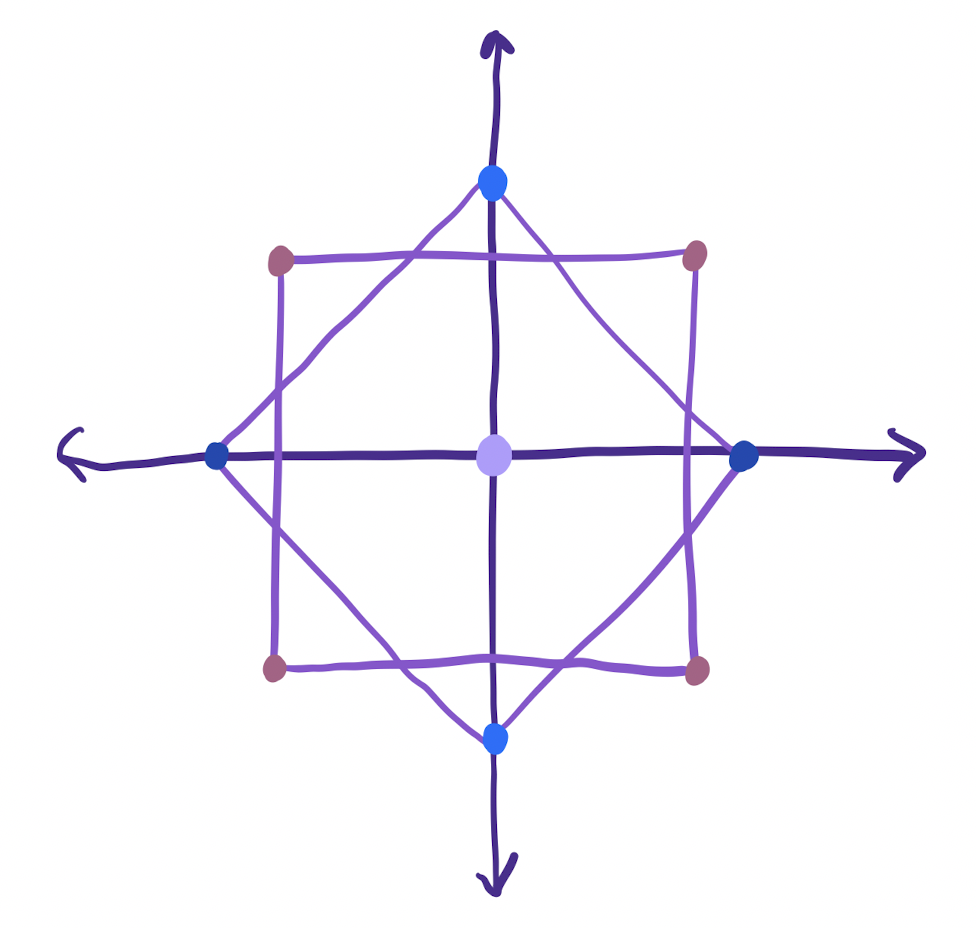
\includegraphics[width=5cm]{Lecture Files and Images/lec17-orbitsofS.png}
\end{center}

\begin{proposition}
The orbits of $G$ form a \emph{partition} of $S.$\footnote{The set can be cut into non-overlapping pieces by the orbits.} In particular, $S$ is the disjoint union of the orbits: $S = \amalg O_i$ where $O_i \cap O_j = \varnothing.$ 
\end{proposition}
\begin{proof}
The orbits clearly cover $S$, since every element $s \in S$ is also an element of $O_s,$ its own orbit. Also, they are disjoint. If $O_s \cap O_{s'} \neq \varnothing,$ then there is some element in their intersection $t = gs = g's'$. Then $s = (g^{-1}g')s',$ which is in $O_{s'}$. So every element of $O_s$ is in $O_{s'},$ and by the same logic $O_{s'} \subseteq O_s.$ Then $O_s = O_{s'}$. So if two orbits have nonempty intersection, they are in fact the same orbit.
\end{proof}

For a finite set, the size of $S$ can be obtained from the sizes of the orbits. 

\begin{corollary}
If $S$ is a finite set, and $O_1, \cdots, O_k$ are the orbits, then 
\[
|S| = \sum_{i = 1}^k |O_i|,
\]
since each of the orbits cover $S$ exactly.
\end{corollary}

In Example \ref{grp action d2}, this gives $9 = 4 + 2 + 2 + 1.$

\begin{qq}
What does each orbit look like?
\end{qq}

For this, we use the notion of a \emph{stabilizer} of an element.

\begin{proposition}
Fix some $s \in S$ and let $H \coloneqq \text{Stab}(s).$ Then there exists a bijection $\varepsilon$ from the quotient group $G/H$ to the orbit of $s,$ $O_s.$ It takes 
\begin{align*}
    G/H &\xrightarrow[]{\varepsilon} O_s \\
    gH &\mapsto gS.
\end{align*}
\end{proposition}

\begin{center}
    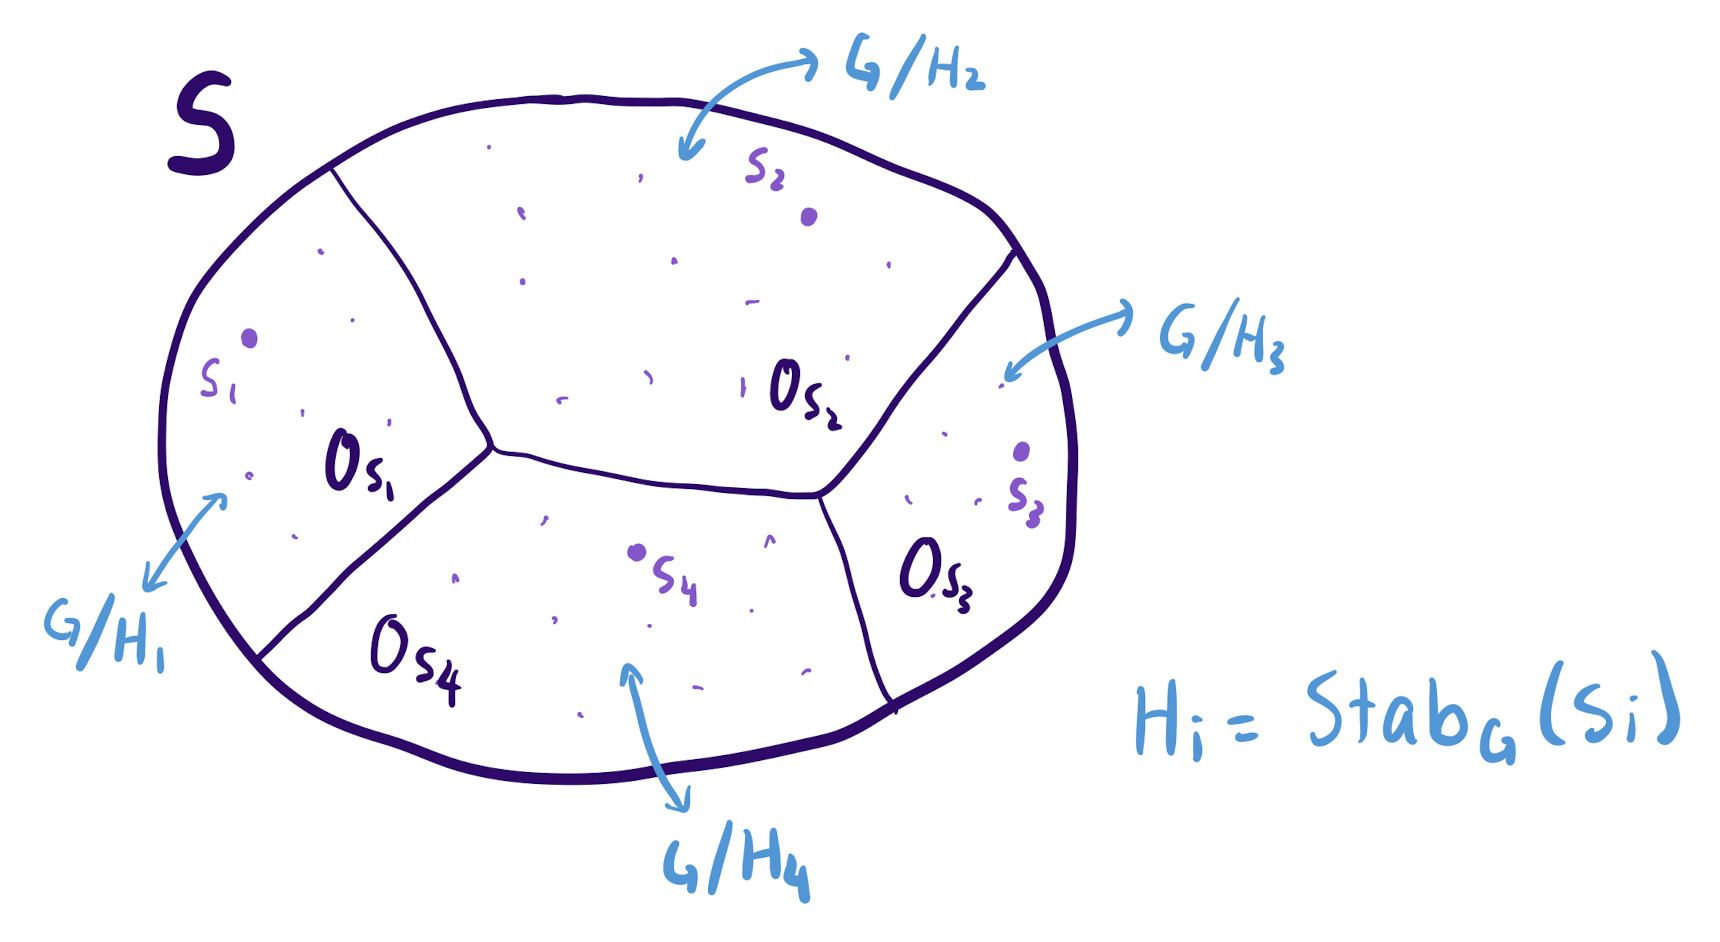
\includegraphics[width=12cm]{Lecture Files and Images/lec17-drawing.png}
\end{center}


\begin{proof}
Consider $g$ and $\gamma$ in $G.$ Then their cosets map to the same element if $gs = \gamma s,$ which is equivalent to saying that $g^{-1}\gamma s = s$. Since $H$ is the stabilizer of $S,$ this means that $g^{-1}\gamma \in H;$ equivalently, $\gamma \in gH.$ Since each of these conditions were equivalent conditions, $gs = \gamma s$ if and only if $\gamma \in gH,$ and thus $\varepsilon$ must be bijective: two elements in $G/H$ map to the same element in $O_s$ if and only if they are the same element.
\end{proof}

\begin{corollary}[Counting Formula for Orbits]
As a result, the number of cosets of $H$, which is the order $|G/H|$, is equal to the size of the orbit of $s,$ since there is a bijective correspondence between them. So 
\[
|O_s| = [G : \text{Stab}(s)].
\]
\end{corollary}

In particular, the size of the orbit of any element $|O_s|$ divides $|G|$ when $G$ is a finite group. We have 
\[
|O_s|\cdot|\text{Stab}(s)| = |G|.
\]

These theorems are similar to the Counting Formula and Lagrange's Theorem from Chapter 2. In particular, let $\mathcal{C}$ be the set of left cosets of a given subgroup $H.$ Then $G$ acts on $\mathcal{C}$; an element $g \in G$ takes $C \mto gC.$ Every coset can be mapped to any other coset by some element of $G.$ For example, $g_1H$ is mapped to $g_2H$ by $g_2g_1^{-1}\in G.$ So there is only one orbit, the entire set $\mathcal{C}$. The stabilizer of the identity coset, which is $eH = H,$ is $\text{Stab}(eH) = H,$ because some element $g \in G$ carries $h \in H$ to $h' \in H$ if and only if $gh = h',$ which implies that $g = h'h^{-1} \in H.$ Thus, the Orbit-Stabilizer Theorem states that 
\[
|G| = |H|[G:H],
\]
since $|H|$ is the stabilizer of the identity in $G/H$ and $[G:H]$ is the size of the identity orbit.


\begin{example}
Consider the subgroup $G \leq SO_3$ consisting of rotational symmetries of a cube centered at the origin. 


\begin{center}
    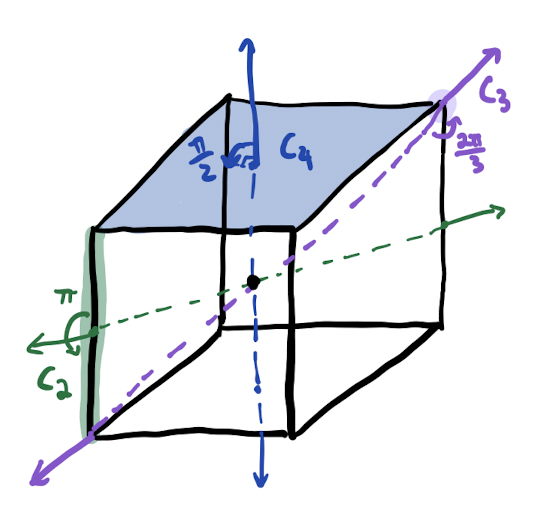
\includegraphics[width=7cm]{Lecture Files and Images/lec17-cube.png}
\end{center}


\begin{itemize}
    \item Let $S$ be the set of faces of the cube; it has order 6 since there are 6 faces. For every face of the cube, there is some element in $G$ mapping it to any other face in the cube ($G$ acts transitively on the faces), so the orbit of a given face is the set of all the other faces, which is $S.$ The stabilizer $\text{Stab}_G(\text{face}) = C_4,$ since a given face, which is a square, is preserved by rotation by $\pi/2$ around the axis through the center of the face. Then 
    \[
    |G| = |S| \cdot |\text{Stab}_G(\text{face})| = 6 \cdot 4 = 24.
    \]
    
    \item Similarly, any vertex can be mapped to any other vertex by some element of $G.$ The stabilizer $\text{Stab}_G(\text{vertex}) = C_3,$ since a vertex is preserved under rotation by $2\pi/3$ around the axis from the vertex to the opposite vertex. Again, 
    \[
    |G| = |\{\text{vertices}\}|\cdot|\text{Stab}_G(\text{vertex})| = 8 \cdot 3 = 24.
    \]
    
    \item Again, $G$ acts transitively on the set of edges. The stabilizer of an edge is $\text{Stab}_G(\text{edge}) = C_2$. Then 
    \[
    |G| =  |\{\text{edges}\}|\cdot|\text{Stab}_G(\text{edge})| = 12 \cdot 2 = 24.
    \]
\end{itemize}

\end{example}

\newpage